\section{Introduction to the Estimation Problem}
\label{sec:M2}

The contents of this lesson cover an introduction to the estimation problems. So, during this session, we will present some basic concepts of estimation design using statistical information. Important concepts, such as {\em a priori} and {\em a posteriori} probabilities, observations, cost functions, or likelihoods will be illustrated through a series of simple examples.

\subsection{Example 1: Bayesian estimation without observations}
\label{subsec:example1}

\begin{problem} 
A food delivery company wants to develop a new service to estimate the time that will elapse from the reception of an order to its delivery to the customer's home.
To do this, the total service or delivery time, $S$, is modelled as a random variable given by the sum of two independent r.v.s:
$$S=T_1 + T_2,$$
where $T_1$ models the time (in minutes) needed to prepare the order and $T_2$ is the shipping time (in minutes).
Analyzing these times the company has characterized r.v.s $T_1$ and $T_2$ with the following probability distributions:

$$p_{T_1}(t_1) = 0.5 \exp{\left[-0.5(t_1 - 10) \right]} \quad \quad  t_1 >10 $$
$$p_{T_2}(t_2) = \frac{0.2}{r} \exp{\left[-\frac{0.2}{r} (t_2-5)\right]} \quad \quad  t_2 >5 $$
where r is the distance (in kilometers) from the company store to the customer's home. 
To estimate the value of $S$, let's start solving the following questions:
    \begin{itemize}
        \item[a)] Knowing the probability distributions of $T_1$ and $T_2$, can we obtain the probability distribution of $S$?
        \item[b)] Knowing the probability distribution of $S$, can we estimate the total delivery time? 
        \item[c)] Which is the optimal estimator for a given cost? 
    \end{itemize}
\end{problem}

\begin{solution} 

\begin{itemize}
\item[a)] Can we obtain the probability distribution of $S$? \\
Computing the distribution of $S$ requires applying a change of random variable in which we have to transform two random variables ($T_1$ and $T_2$) into a new variable ($S$). Since $S$ is the sum of two independent random variables, we know that their distribution will be given by the convolution of the distributions of $T_1$ and $T_2$: 
$$ p_S(s) = p_{T_1} (t_1=s) \ast  p_{T_2} (t_2=s)  = \int  p_{T_1} (t_1=s)  p_{T_2} (t_2=s-t_1) d t_1   $$
after some mathematical manipulations (the complete mathematical development is left as an exercise), we can see that $p_S(s)$ is given by the following expression (see Figure \ref{Fig_ps}):
$$ p_S(s) = \left(0.5 + \frac{0.2}{r}\right) \left(s -15\right) \exp{\left[-\left(0.5 + \frac{0.2}{r}\right) \left(s-15\right)  \right]}   \quad  s >15$$

\begin{figure}[!t]
\begin{center}
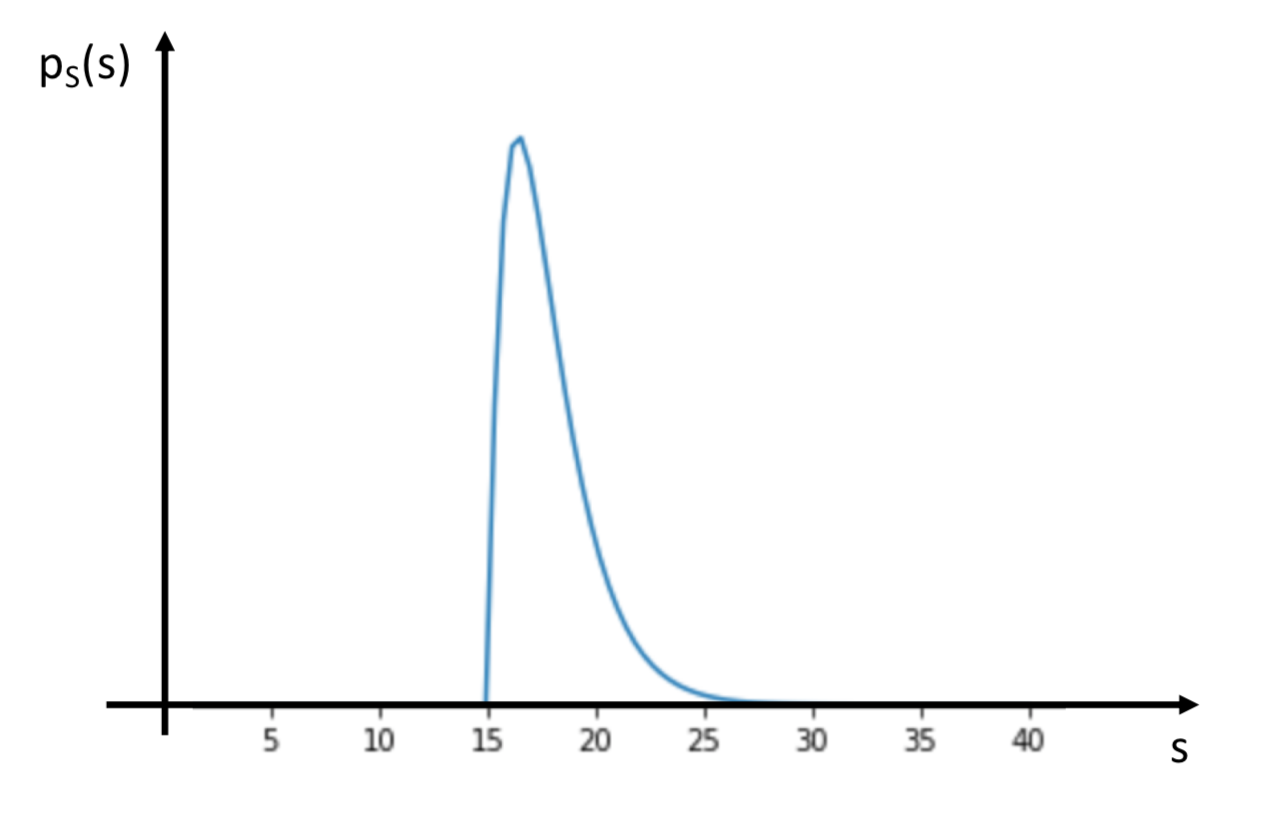
\includegraphics[scale=.25]{Figures/Fig_MC1_1.png}
\caption{Representation of the probability distribution of $S$ for $r=1$.}
\label{Fig_ps}
\end{center}
\end{figure}
\vspace{0.2cm}
\item[b)] Can we now estimate the total delivery time?\\
Let's consider that we receive an order to be delivered to one kilometer of distance ($r=1$Km), so we have that 
$$ p_S(s) = 0.7 \left(s -15\right) \exp{\left[-0.7 \left(s-15\right)  \right]}   \quad  s >15.$$
Knowing this distribution, we can know which values of $S$ are most probable and which values are completely unlikely; for instance, analyzing Figure \ref{Fig_ps}, we can realize that it is quite likely that $S$ is between $15$ and $20$, whereas it is impossible that it is lower than $15$, and it is almost impossible that it is greater than $30$. So,  in light of the distribution of $S$, we can estimate the total delivery time considering different criteria (see Figure \ref{Fig_ps_s1_s2}):

\begin{figure}[!t]
\begin{centering}
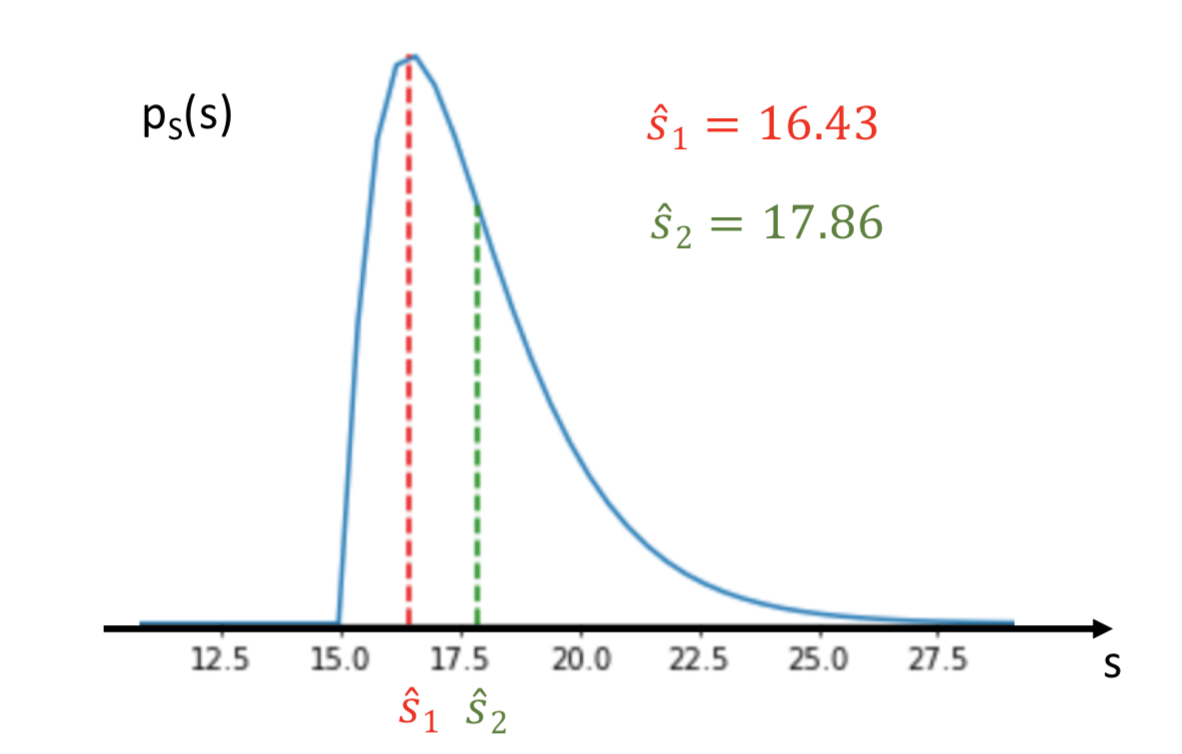
\includegraphics[scale=.25]{Figures/Fig_MC1_2.png}
\caption{Some possibles estimators of $S$ analyzing $p_S(s)$.}
\label{Fig_ps_s1_s2}
\end{centering}
\end{figure}

\begin{itemize}
\item One could consider that a good estimation could be given by the most likely value of $S$, that is, by the mode of $S$:
$$ \hat{s}_1  = {\arg\max_s}  p_S(s) $$
and we can compute this value by deriving $p_S(s)$ and setting the result to zero:

$$  \left.\frac{\partial p_S(s)}{\partial s} \right|_{s = \hat{s}_1} = 0.7 \exp{\left[-0.7 \left(\hat{s}_1 -15\right) \right]} - 0.7^2 \left(\hat{s}_1 -15\right) \exp{\left[-0.7 \left(\hat{s}_1 -15\right)  \right]} =0$$
Now, we can cancel the term\footnote{Note that by cancelling this term we are skipping the solution $\hat{s}_1 \rightarrow \infty$, but analyzing the shape of $p_S(s)$ we can check that this root is a minimum.} $0.7\exp{\left[-0.7 \left(\hat{s}_1 -15\right) \right]}$ and get:

$$ 1 - 0.7( \hat{s}_1 -15) =0$$
$$ \hat{s}_1  = 15 + \displaystyle \frac{1}{0.7}= 16.43~ {\rm min.}$$
To complete this calculation, we have to check that this solution is a maximum (the derivative only guarantees returning relative extremes or saddle points). We can do this either analyzing the shape of $p_S(s)$ or checking that the second derivative is negative.
\item Another possible estimation could be given by the expected value of $S$,
$$  \hat{s}_2 = \mathbb{E}\{S\} = \int s p_S(s) ds =  \int_{15}^{\infty} 0.7 s \left(s -15\right) \exp{\left[-0.7 \left(s-15\right)  \right]} ds $$
and solving this integral by parts, we have
$$ \hat{s}_2 =   15 + \displaystyle \frac{2}{0.7}=17.86~{\rm min.}$$
\item Or we could even raise other estimators, such as the median of the distribution or the 25\% or 75\% percentiles. 
\end{itemize}

Finally, it is important to bear in mind that regardless of the estimator we use, we probably have an estimation error (it is practically impossible for the estimated value to coincide with the actual one) and the error of each estimator will indicate us which estimator is more adequate. %In fact, if we know how our problem is going to measure the different errors (what the cost function gives us), the ideal is for us to design the estimator trying to minimize this cost. 
In fact, in this unit we will pursue as a design criterion the minimization of the mean value of a cost criterion that establishes how we should penalize different kinds of errors.

\vspace{0.2cm}
\item[c)] How can we find the optimal estimator for a given cost? 
For the design of the estimator, the food delivery company wants to minimize the following cost function (see Figure \ref{Fig_MC1_5}):
\begin{equation} 
c(\hat{s},s) = \begin{cases}
0.005|s-\hat{s}| & {\rm if} \quad \hat{s}>s\\
0.1|s-\hat{s}|  & {\rm if} \quad \hat{s}<s 
\end{cases} \nonumber
\end{equation} 

%{\color{red} Podemos dar un significado a este coste? Perdidas en Keuros? Pero en ese caso siempre pierde... y no tiene sentido definir costes negativos que serían beneficios.... Ponemos unas ganancias máximas y esto son perdidas sobre esas ganacias....???}

\begin{figure}[!t]
\begin{tabular}{m{.1\textwidth}m{.5\textwidth}m{.4\textwidth}}
&\raisebox{-18ex}{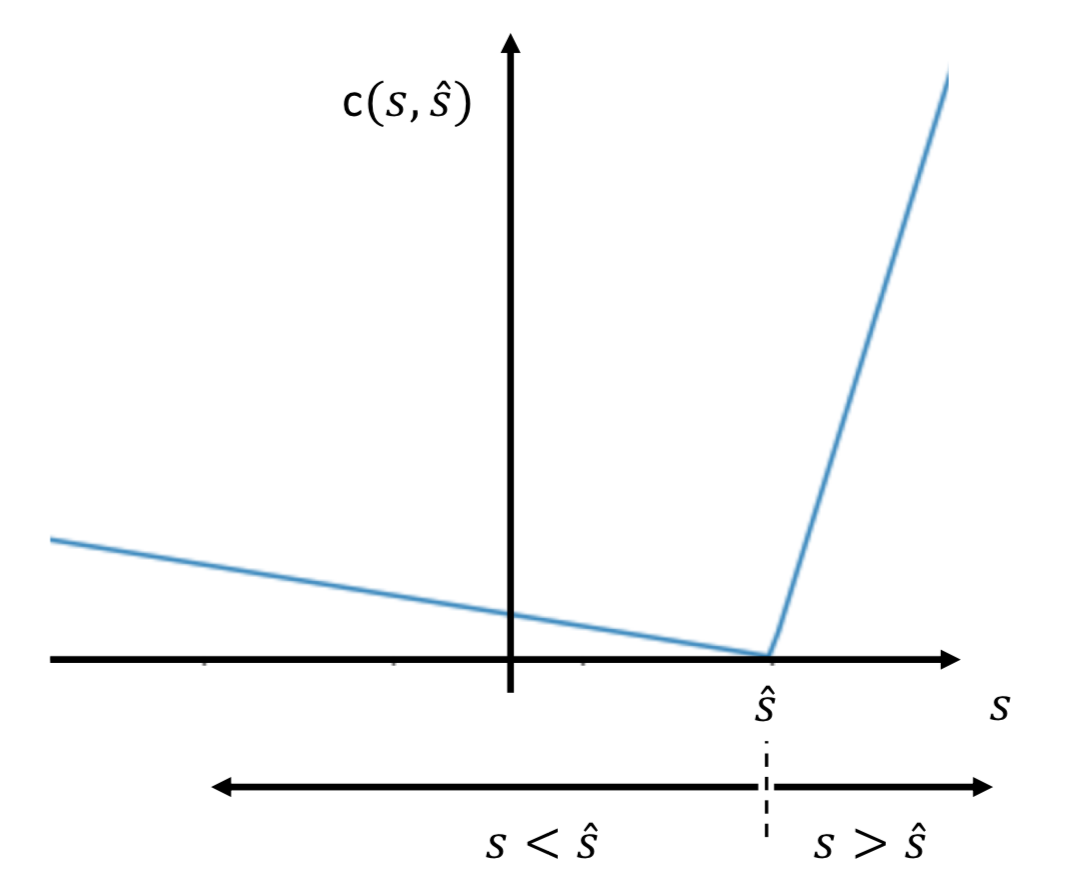
\includegraphics[scale=.25]{Figures/Fig_MC1_5.png}}&
 \begin{equation} 
c(\hat{s},s) = \begin{cases}
0.005|s-\hat{s}| & {\rm if} \quad \hat{s}>s\\
0.1|s-\hat{s}|  & {\rm if} \quad \hat{s}<s 
\end{cases} \nonumber
\end{equation} 
\end{tabular}
\caption{Asymmetric cost function to be minimized during the estimator design.}
\label{Fig_MC1_5}
\end{figure}

As any cost function, this cost function indicates how we have to penalize the fact that the estimated value differs from the actual value of $S$. However, unlike typical cost functions, this is an asymmetric cost function (see Figure \ref{Fig_MC1_5}), that is, it applies different penalties in case of overestimating the values of $S$ ($\hat{s} >s $) or underestimating them ($\hat{s} <s $). In this way, this cost function is indicating that if the order arrives before the time we have estimated it will penalize less than in case the customer has to be waiting longer than expected, i.e., if our  order takes longer to arrive than we have estimated. In this case, using the mean or median of $S$ is not the most appropriate estimator, and we should choose a value higher than the expected one. I.e., since subestimations of the actual time of delivery are highly penalized, we should try to be conservative and produce estimators that are only rarely exceeded. So, it is possible that a value around the 70\%-80\% percentile of the $p_S(s)$ distribution is close to the estimator we are looking for.


Reviewing the expression of the cost function to be minimized, we can see that the cost value depends both on the estimator $\hat{s}$ and on the random variable to be estimated $S$. So, as the cost function is a function of a random variable, it is itself another random variable. For this reason, we are going to denote it as $ C = c(\hat{s},S)$.

\begin{figure}[!t]

\begin{tabular}{m{.5\textwidth}m{.5\textwidth}}
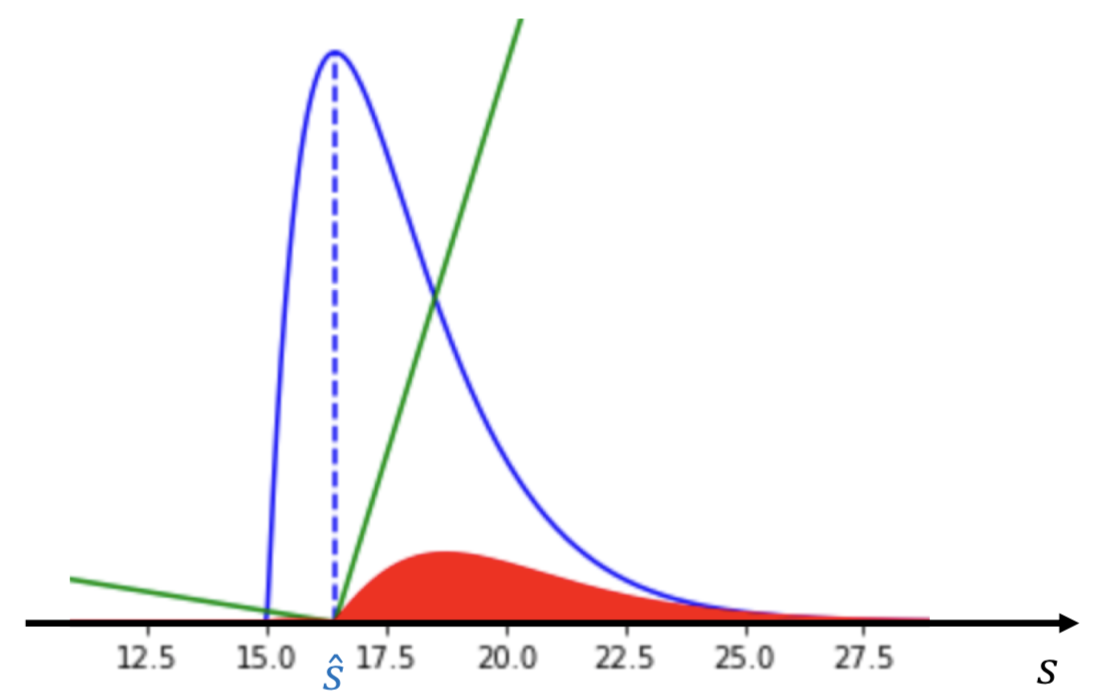
\includegraphics[scale=.3]{Figures/Fig_MC1_6.png}&
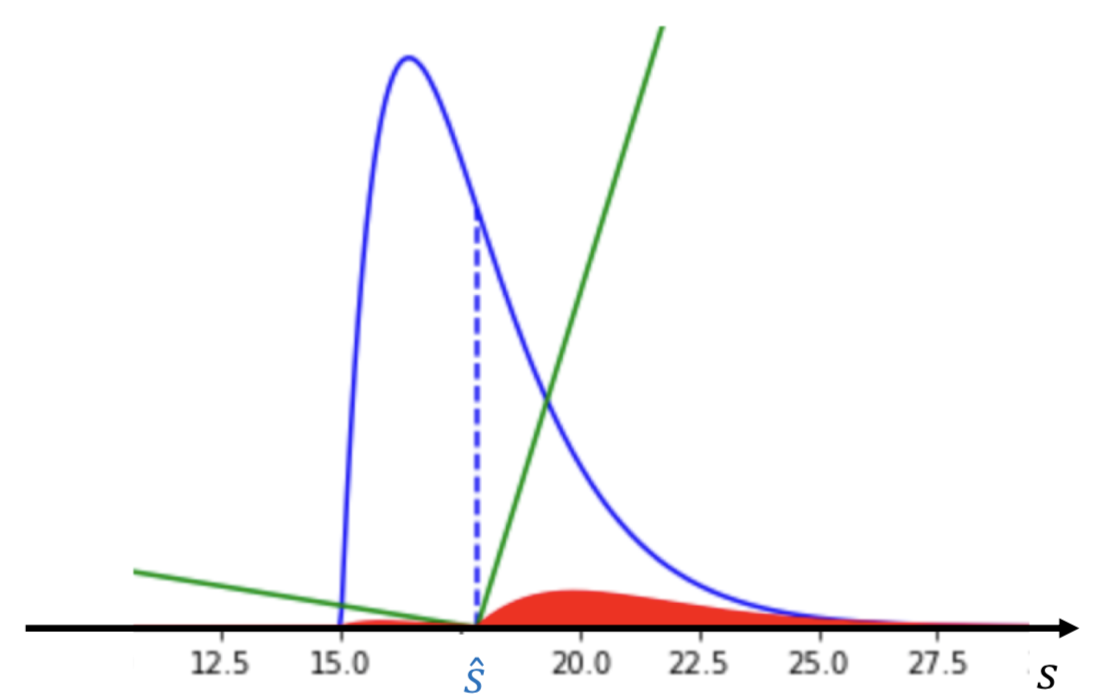
\includegraphics[scale=.3]{Figures/Fig_MC1_7.png}\\
(a) $\hat{s} = 16.43 \quad \mathbb{E}\{C\} = 0.23$ &
(b) $\hat{s} =  17.86 \quad  \mathbb{E}\{C\} = 0.12 $ \\
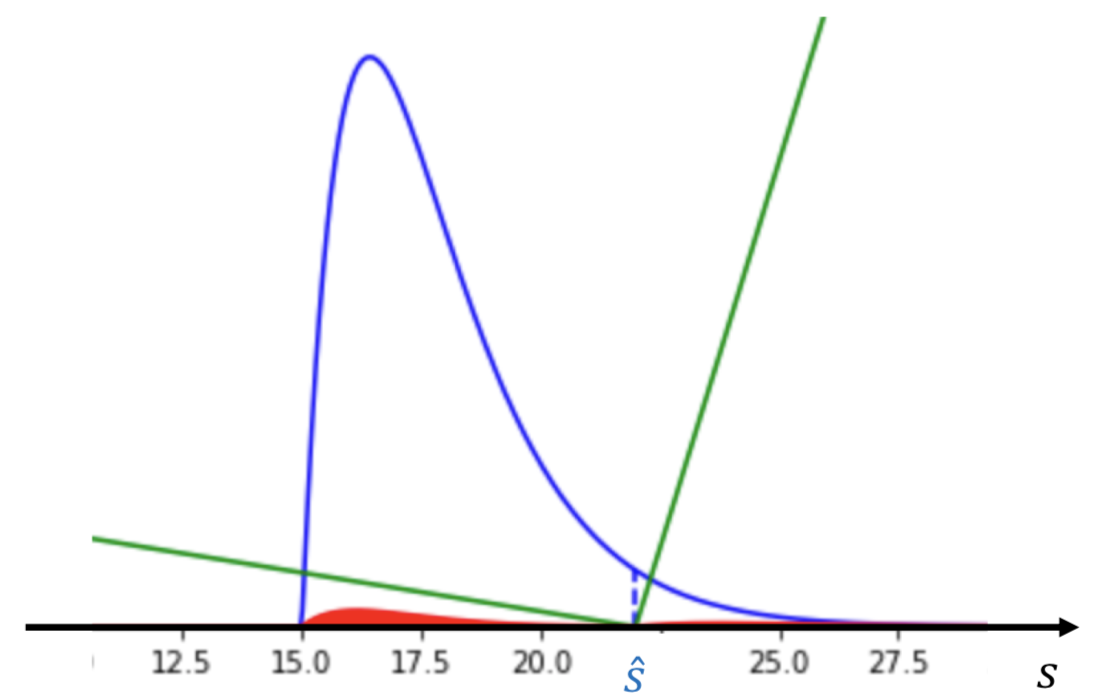
\includegraphics[scale=.3]{Figures/Fig_MC1_8.png}&
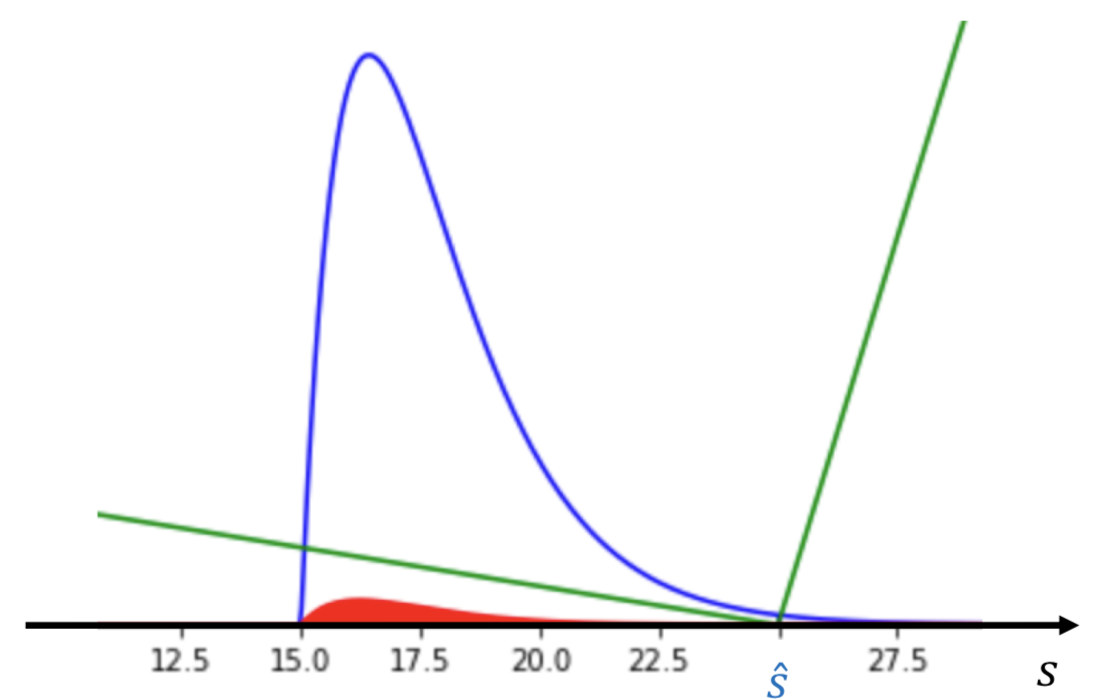
\includegraphics[scale=.3]{Figures/Fig_MC1_9.png}\\
(c) $\hat{s} = 22  \quad \mathbb{E}\{C\}= 0.04$ &
(d) $\hat{s} =  25 \quad \mathbb{E}\{C\}=0.05$ \\
\multicolumn{2}{c}{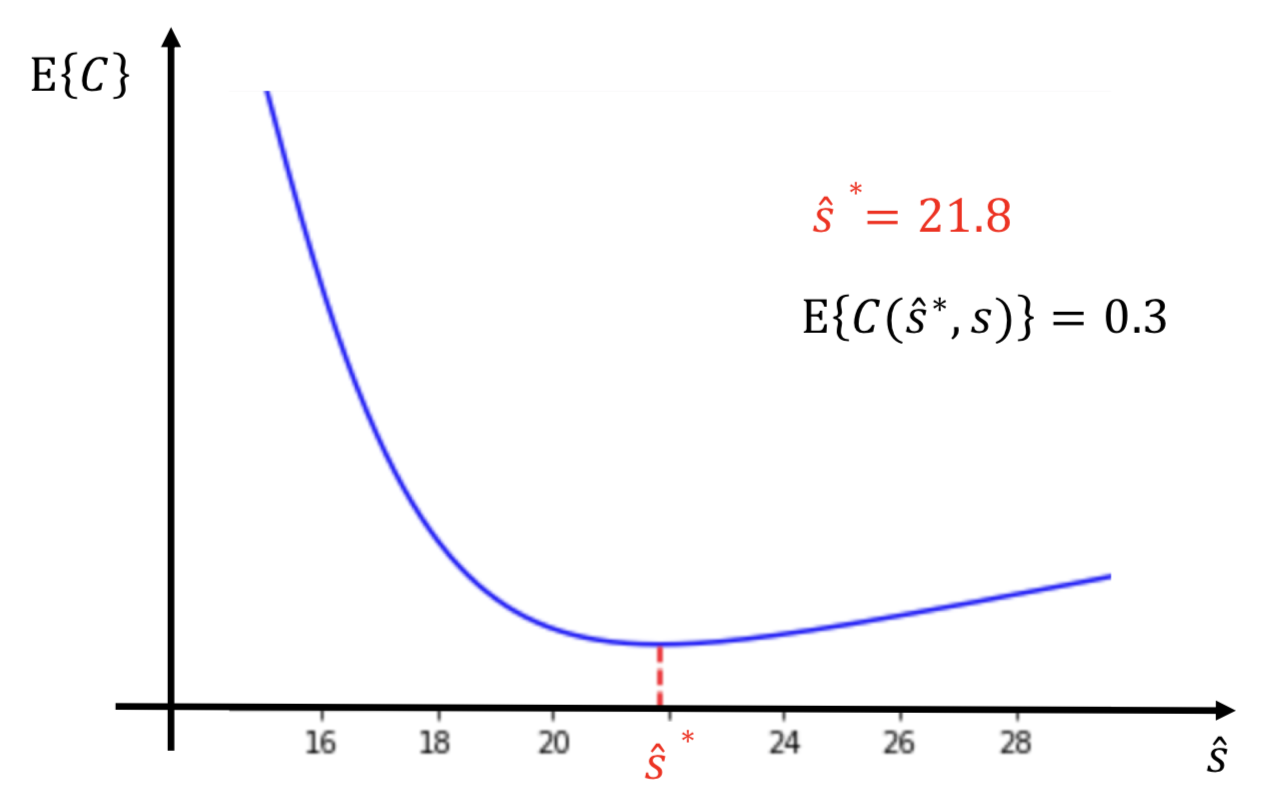
\includegraphics[scale=.25]{Figures/Fig_MC1_10.png}}\\
\multicolumn{2}{c}{(e) Evolution of the mean cost with the value of $\hat{s}$}
\end{tabular}
\caption{Process of minimization of the mean cost for different values of the estimator.}
\label{Fig_MC1_6_9}
\end{figure}

When we wanted to find the value of the estimator that minimizes the cost $C$, we would have to find the value of the estimator which minimizes the expected cost or the mean cost. So, the optimum estimator would be given by:
$$ \hat{s}^{*} = \arg\min_s~ \mathbb{E}\{C\} = \arg\min_{\hat{s}}~ \mathbb{E}\{c(\hat{s},S)\}$$
where the mean cost is computed as:
$$\mathbb{E}\{c(\hat{s},S)\} = \int c(\hat{s},s) p_s(s) ds$$


For each possible value of the estimator, we will get a different mean cost, and we will have to select the estimator value that provides the minimum mean cost. Fig \ref{Fig_MC1_6_9} shows the average cost for different values of the estimator for the given asymmetric cost function. In fact, Subfigures \ref{Fig_MC1_6_9}(a)-(d) show how the mean cost is computed for different values of the estimator; note that the mean cost is computed as the area resulting from multiplying the distribution $p_S(s)$ by the cost function $c(\hat{s},S)$, and, as different values of the estimator, $\hat{s}$,  will place the cost function in different positions, this process will result in different mean costs. If we directly compute the mean cost for any possible value of $\hat{s}$ we would obtain a curve similar to that shown in Subfigure \ref{Fig_MC1_6_9}(e) and $\hat{s}^{*}$ would be the value of $\hat{s}$ which minimizes it. In this case, we can see that the optimum  estimator would be $\hat{s}^{*} = 21.8$ min and it generates a mean cost of $0.3$.


\end{itemize}
\end{solution}

\subsection{Example 2: Bayesian estimation with observations}
\label{subsec:example2}

\begin{problem}
To obtain a more accurate estimation of the delivery time, the company has improved the food preparation process, so that it is able to know the exact time it will take to prepare the order $T_1=t_1$. 

When we want to estimate the value of $S$ without observations, the only distribution which provides information about the value of $S$ is $p_S(s)$; however, when we have additional information such as knowledge of the value of $t_1$ (observation), including this information in our estimation problem makes the estimation of $S$ easier (more accurate). Adding this knowledge (observation) to the estimation task implies using the posterior distribution of $S$, $p_{S|t_1}(s|t_1)$, instead of using $p_S(s)$.

To solve the estimation problem in this new scenario, let's try to answer the following questions:
 \begin{itemize}
\item[a)] Can we obtain the probability distribution of $S$ given the value $T_1=t_1$?
\item[b)] Can we estimate the total delivery time for a given value $T_1=t_1$? 
\item[c)] Given a cost function to be optimized, which is the optimal estimator for a given value $T_1=t_1$? 
    \end{itemize}
\end{problem}

\begin{solution}
\begin{itemize}
\item[a)] Can we obtain the probability distribution of $S$ given the value $T_1=t_1$?\\
The calculation of the posterior distribution of $S$ can be done by applying the following r.v change\footnote{Note that as we are calculating the distribution of $S$ given $T_1$, the value of $T_1$ is known ($T_1=t_1$).}:
$$S = t_1 + T_2$$
so, $p_{S|t_1}(s|t_1)$ can be obtained by shifting the distribution of $p_{T_2}(t_2)$ to the position of $t_1$, i.e.,
$$p_{S|t_1}(s|t_1)=p_{T_2}(t_2=s-t_1) =
\frac{0.2}{r} \exp{\left[-\frac{0.2}{r} (s-t_1-5)\right]} \quad \quad  s >t_1 +5$$
%\begin{figure}[!h]
%\begin{center}
%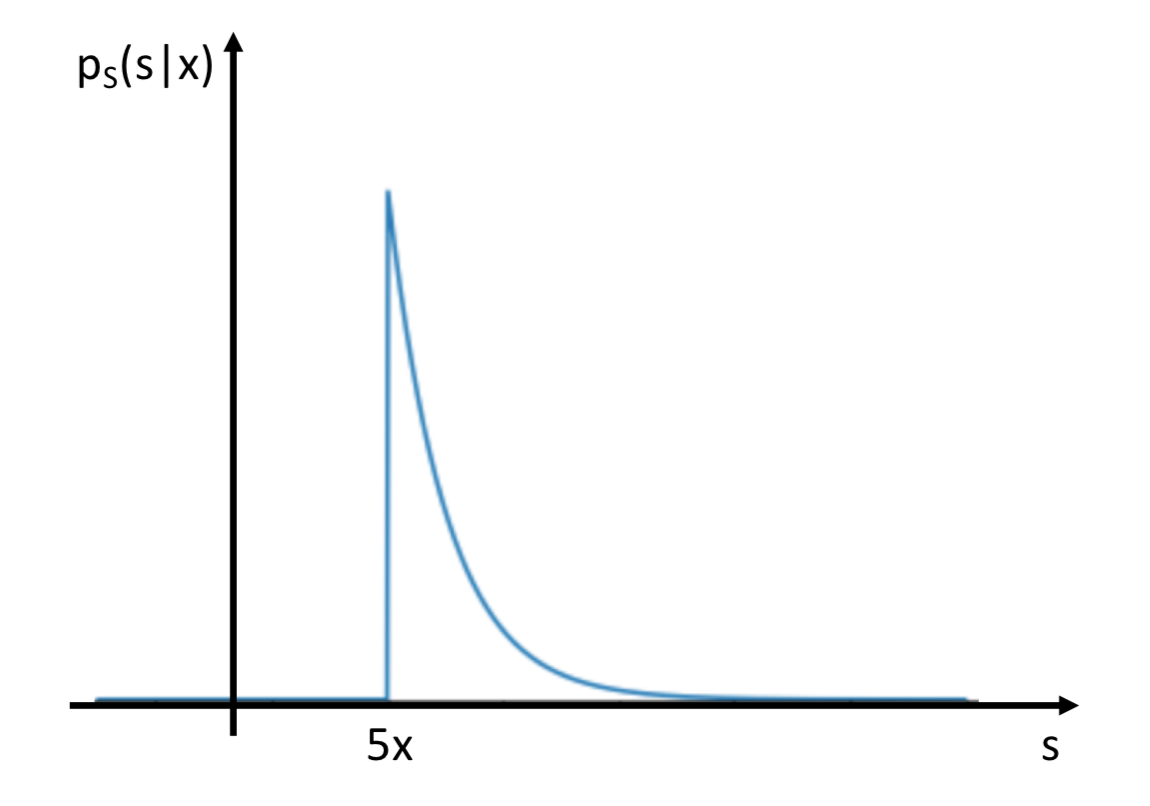
\includegraphics[scale=.25]{Figures/Fig_MC1_11.png}
%\end{center}
%\end{figure}


\item[b)] Can we estimate the total delivery time for a given value $T_1=t_1$? 

To answer this question, let's consider that a customer is calling the food company to place an order from a distance of one kilometer ($r=1$Km), and in this moment and for this order the preparation time is $t_1=12$ minutes. So we have:

$$p_{S|t_1}(s|t_1)=p_{T_2}(t_2=s-t_1) =
0.2 \exp{\left[-0.2 (s-17)\right]} \quad \quad  s >17$$

and, examining this distribution (see Figure \ref{p_S_x2}), we can consider different estimators such as the maximum of the distribution, which is $\hat{s}_1=17$ min., or the expected value of $S$ given $t_1=12$, which can be computed (by solving the integral by parts) as:

$$ \hat{s}_2= \mathbb{E}\{S|t_1=12\} = \int s p_{S|t_1}(s|t_1) ds = 17+\frac{1}{0.2} = 22 {\rm min.}$$

\begin{figure}[!t]
\begin{center}
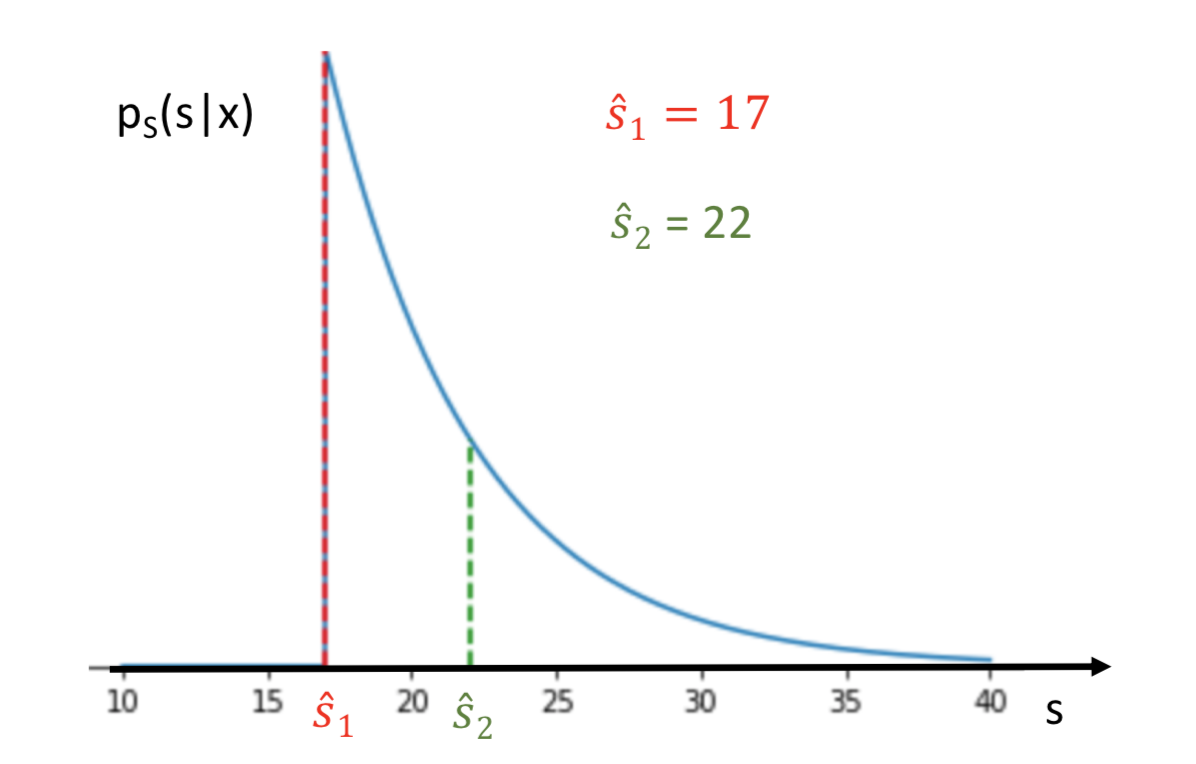
\includegraphics[scale=.25]{Figures/Fig_MC1_12.png}
\caption{Some possible estimators of $S$ given that $t_1=12$.}
\end{center}
\label{p_S_x2}
\end{figure}

For any value of the observation, the posterior distribution of $S$ will change (in this case, the $ p_{S|t_1}(s|t_1)$ will be shifted) and the value of the estimator will depend on the observation value ($t_1$). If we want to obtain a general expression for these estimators (for any value of $t_1$), we can directly compute both the maximum and the mean by using the expression of the posterior for any value of $t_1$ (we are still considering $r=1$):
$$ p_{S|t_1}(s|t_1) = 0.2 \exp{\left[-0.2 (s-t_1-5)\right]} \quad \quad  s >t_1 +5$$

For example:

\begin{itemize}
\item If we consider that the mode of $ p_{S|t_1}(s|t_1)$ could be an adequate estimator, the estimator will be:
$$ \hat{s}_1  = {\arg\max_s}  p_{S|t_1}(s|t_1) $$
In this case, as $p_{S|t_1}(s|t_1) $ is a decreasing function for $s >t_1 +5$, its maximum is 
$$\hat{s}_1 = t_1 +5.$$

\item We can also consider that the expected value of $S$ given $t_1$ is a good estimator. In this case (computing the integral by parts):
$$\hat{s}_2= \mathbb{E}\{S|t_1\} = \int s p_{S|t_1}(s|t_1) ds = 5 + t_1 +\frac{1}{0.2} = 10+t_1$$
\end{itemize}


However, in order to decide which estimator is best, we need, as before, to define which cost function we want to minimize.

\item[c)] Given a cost function to be optimized, which is the optimal estimator for a given value $T_1=t_1$? 

Again, when we are designing an estimator we may want to design it in such a way that it minimizes the mean value of a given cost function. Now, as we are now working with observations, our goal will be finding the optimal estimator for any observed value (for any given value of $T_1=t_1$). 

Thus, we can now find the optimum estimator by 
$$ \hat{s}^{*} = \arg\min_s~ \mathbb{E}\{c(\hat{s},S)|t_1\}$$
where 
$$\mathbb{E}\{c(\hat{s},S)|t_1\} = \int c(\hat{s},s) p_{S|t_1}(s|t_1)  ds$$


\begin{figure}[!t]
\begin{tabular}{m{.5\textwidth}m{.5\textwidth}}
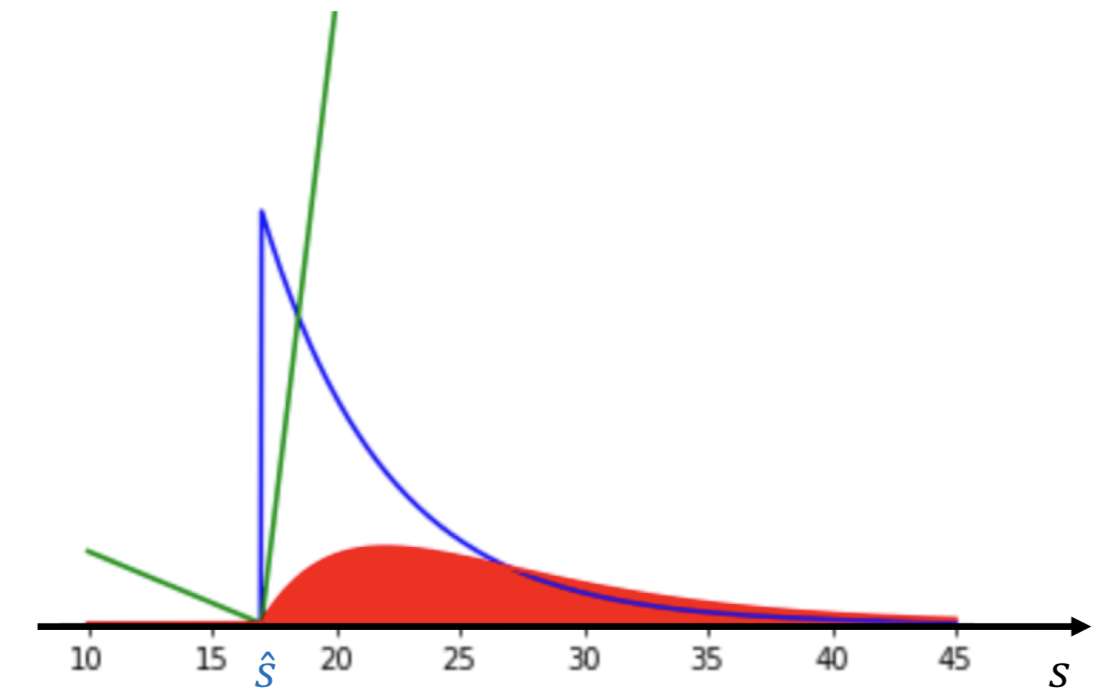
\includegraphics[scale=.3]{Figures/Fig_MC1_13.png}&
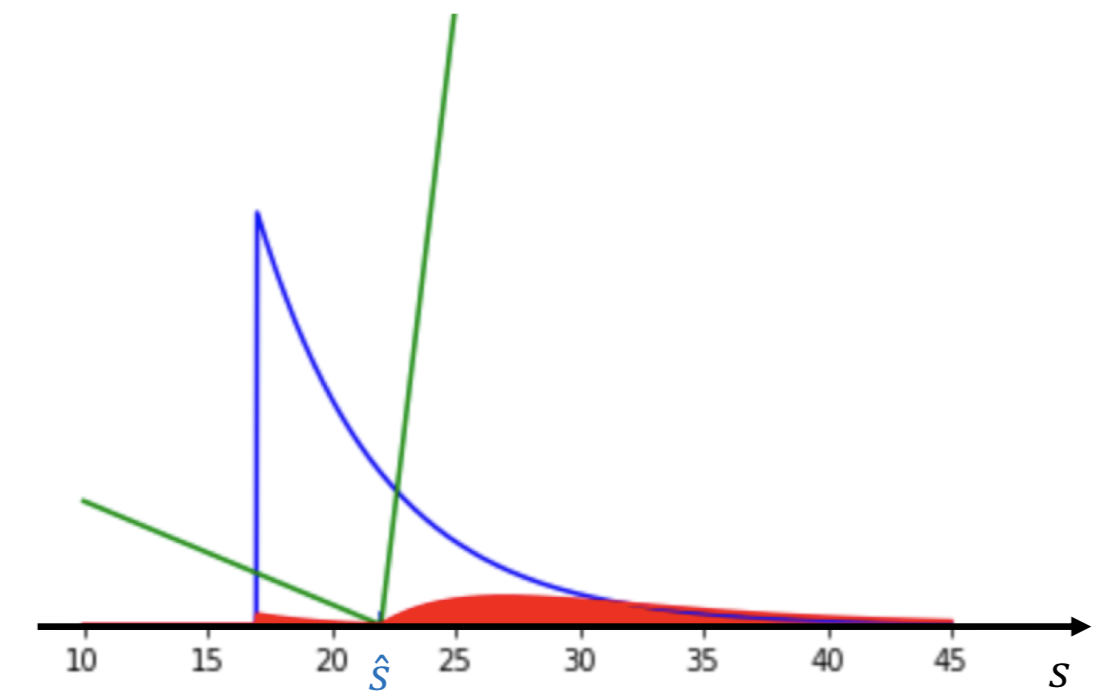
\includegraphics[scale=.3]{Figures/Fig_MC1_14.png}\\
(a) $\hat{s} = 17$ min. and  $ \mathbb{E}\{c(\hat{s},S)|x\} = 0.999$  &
(b) $\hat{s} = 12$ min. and $ \mathbb{E}\{c(\hat{s},S)|x\} = 0.385 $ \\
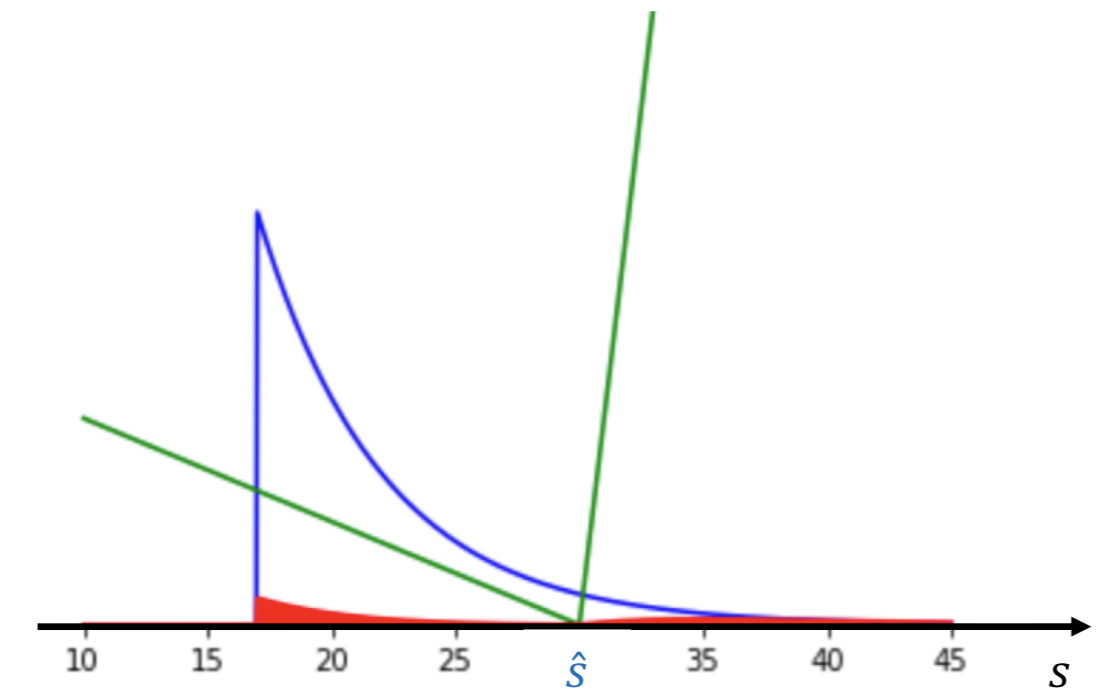
\includegraphics[scale=.3]{Figures/Fig_MC1_15.png}&
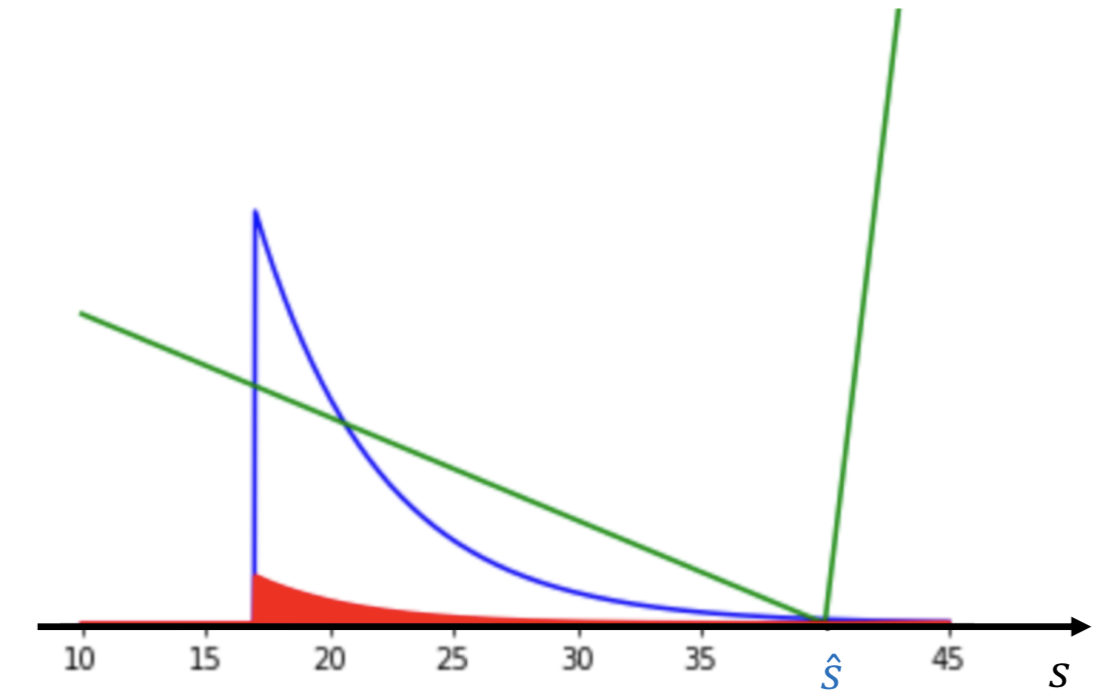
\includegraphics[scale=.3]{Figures/Fig_MC1_16.png}\\
(c) $\hat{s} = 30$ min. and  $\mathbb{E}\{c(\hat{s},S)|x\}= 0.158$ &
(d) $\hat{s} = 40$ min. and  $\mathbb{E}\{c(\hat{s},S)|x\}=0.169$ \\
\multicolumn{2}{c}{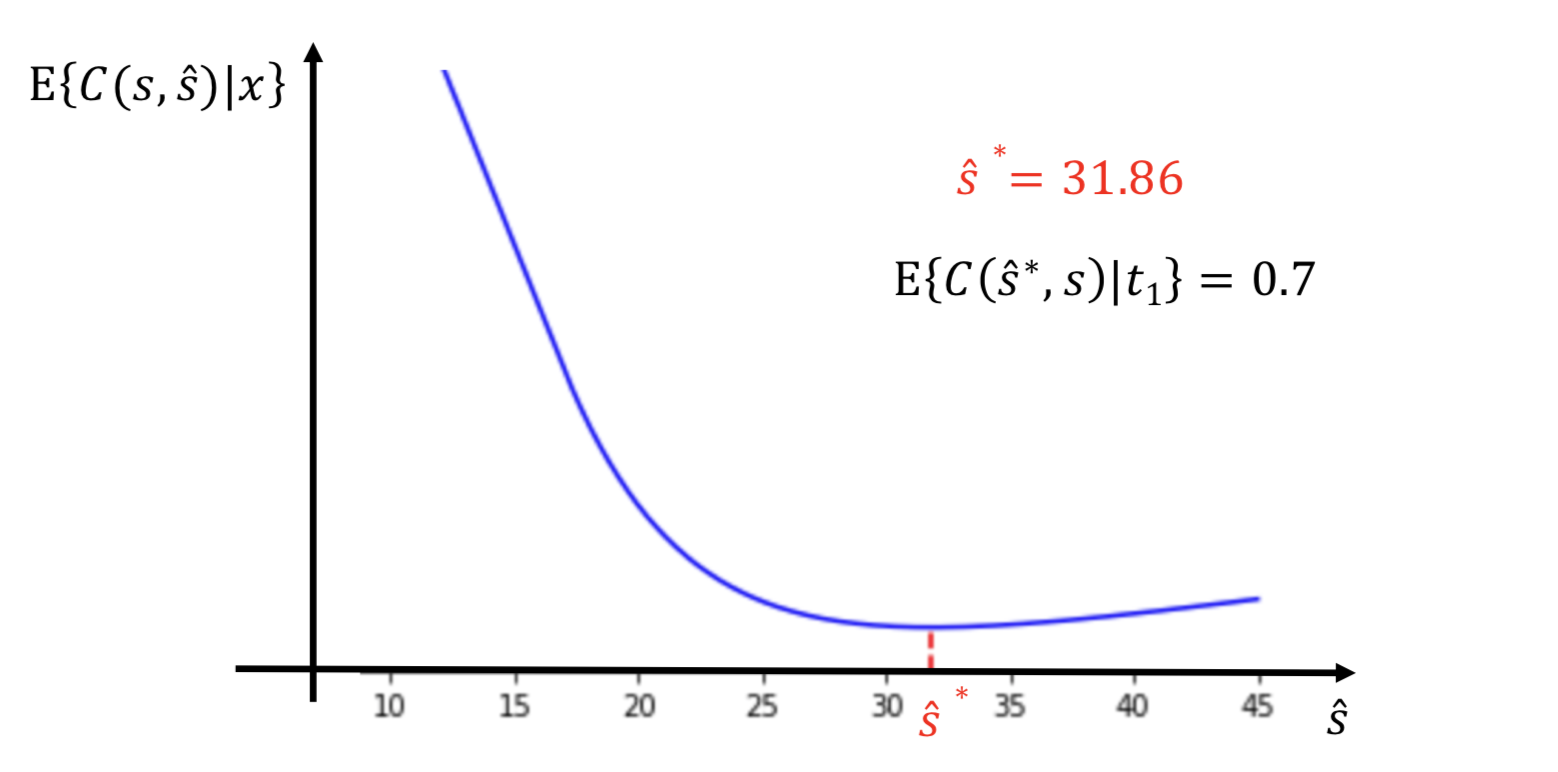
\includegraphics[scale=.25]{Figures/Fig_MC1_17.png}}\\
\multicolumn{2}{c}{(e) Evolution of the mean cost given  $t_1$ with the value of $\hat{s}$}
\end{tabular}
\caption{Process of minimization of the mean cost given $t_1$ for different values of the estimator.}
\label{Fig_MC1_13_17}
\end{figure}

Once again, each possible value of the estimator will provide a different mean cost for a given value of $t_1$ and our goal will be to select the estimator that minimizes said mean cost. 
Summarizing our example problem:
\begin{itemize}
\item An order is placed to be shipped to a distance of one kilometer ($r=1$Km);
\item For this order the preparation time is $t_1=12$ minutes;
\item We want to minimize the asymmetric cost function used in Problem \ref{subsec:example1}(c);
\end{itemize}
Fig \ref{Fig_MC1_13_17} shows the procedure of minimizing the mean cost given $t_1=12$. Subfigures \ref{Fig_MC1_13_17}(a)-(d) plot the conditional mean costs for different values of the estimator and Subfigure \ref{Fig_MC1_13_17}(e) illustrates the mean cost as a function of $\hat{s}$. Analyzing these figures, we can check that the optimum estimator value is $\hat{s}^{*} = 31.86$ min and it generates a mean cost (given that $t_1 = 12$) of $0.7$.

%{\color{red} Creo que dejar lo siguiente estarí bien si pudieramos calcular la expresión analítica de $\hat{s}^{*}$ para cualquier $t_1$ y luego el coste medio global... Como analíticamente no es sencillo, no sé si es bueno dejarlo o no.... Otra cosa es hacerlo en python y poner la gráfica o algo asi.... En cualquier caso creo que habría que incluir indicando que el estimador es una función de las observaciones y su diseño consiste en encontrar esta función...}
Finally, it is important to note that the involved mean cost is for a value of $t_1=12$. If we wanted to compare this cost with that incurred by the estimator designed without observations, we would have to compute the optimum estimator and its mean cost (given the observation) for any value of $t_1$ and average these costs taking into account the probability of each $t_1$ value. %That is, we would have to compute the global mean cost of 

%Applying this procedure, we are computing an estimator for each value of $X=x$ and minimizing the mean cost given the observation, but are we minimizing the total cost?. The answer to this question is ``yes'', since from this relationship:
%\begin{eqnarray}
%\mathbb{E}\{c(\hat{S},S)\}  & =&  \int \int c(\hat{s},s) p_{S,X}(s,x)  ds dx \nonumber \\
%&=& \int \left[ \int c(\hat{s},s) p_{S|x}(s|x)  ds \right]  p(x) dx \nonumber  \\
%&=& \int \left[ \mathbb{E}\{c(\hat{s},S)|x\}  \right]  p(x) dx \nonumber  
%\end{eqnarray}
%allows us to claim that minimizing the mean cost given the observation for any value of $x$, we are minimizing the overall mean cost.
\end{itemize}
    
\end{solution}

%\subsection{Example 3: Maximum likelihood estimation}

%\begin{problem}
%Communication channel with gaussian noise
%$$X = S +N$$


%$$p_N(n) = G(0, v_N)$$

%We transmit signal $S$ and in the receptor we observe $X$, our goal is to estimate the transmitted value ($S$) with the observation of the signal in the receptor ($X$).
%\begin{itemize}
%\item[a)] Without additional information, can we estimate the value of $S$?
%\item[b)] Could we design a bayesian estimator (the optimum estimator for a given cost)?
%\end{itemize}
%\end{problem}

%\begin{solution}
%\begin{itemize}
%\item[a)] Without additional information, can we estimate the value of $S$?
%With the given information, the only distribution that we can easily compute is the likelihood of $S$, that is, the distribution of $X$ given $S$. This distribution can be computed sifting the distribution of $N$ to the position of $S$, i.e.,

%$$p_X|s(x|s)= p_N(n= x-s) = G(s, v_N)$$

%INCLUIR FIGURA LIKELIHOOD


%This distribution indicates the probability of observing $X=x$ for a transmitted value of $S=s$. Imagine that our observation is $x=1$, then, we could use the likelihood to calculate the probability of observing $x=1$ for any value of $s$

%INCLUIR FIGURA LIKELIHOOD en funcion de s para x=1.

%At the light of this figure, what value $S$ has been transmitted? We can say 

%\item[b)] Could we design a bayesian estimator (the optimum estimator for a given cost)?
%\end{itemize}
%\end{solution}